% Chapter 5: Discussion
This chapter discusses what the results in Chapter~\ref{ch:results} mean for the thesis argument. The empirical findings do not support a broad claim that all measured signal characteristics raise returns consistently. They point instead to a conditional result: among \textit{Hype Intensity}, \textit{Urgency Index}, and \textit{Instruction Density}, evidence is clearest for \textit{Urgency Index}, especially when the target asset is small enough to move but still active enough for the effect to be measured. This discussion therefore connects the results with the theoretical framework from Chapter~\ref{ch:literature-framework}, while keeping causal interpretation separate from prediction.

Hypothesis 1 receives partial support, but this support is concentrated in one of the three signal characteristics rather than spread evenly across all of them. The strongest finding is the small-cap estimate for \textit{Urgency Index} in Table~\ref{tab:stratified-ate-results}. Under the DML specification, the coefficient is 0.0301 and statistically significant at the 1\% level ($p < 0.001$). This estimate is large compared with the other significant coefficients reported in Chapter~\ref{ch:results}, especially the other urgency estimates, although the treatment variables are not all measured on the same scale. Since the outcome is the \textit{10-Minute Logarithmic Return} and \textit{Urgency Index} is scaled from 0 to 1, a 10 percentage point increase in the uppercase share of the signal corresponds to about 0.003 log-return units, or roughly a 0.30\% higher price return over ten minutes, holding the model's observed controls constant. This is the clearest evidence that urgent wording can work as a short-term coordination trigger.

This makes the small-cap urgency result the main empirical contribution of the discussion. The estimate is not only statistically significant, but also substantively visible in relation to the other reported effects. Its size suggests that the style of the reveal message can matter during the short period when participants are deciding whether to buy immediately. The scale caveat remains important, since \textit{Instruction Density}, \textit{Hype Intensity}, and \textit{Urgency Index} are constructed differently. Even with that caution, the result gives the strongest support to the thesis claim that the public signal itself is part of the manipulation mechanism.

The result still narrows rather than fully confirms Hypothesis 1. The estimate does not mean that all urgent messages raise prices, or that urgency works in every part of the cryptocurrency market. Chapter~\ref{ch:results} reports no comparable positive effect in the micro-cap, mid-cap, or large-cap strata. The safer interpretation is therefore that urgency plays a positive role in the small-cap segment, while the wider evidence remains conditional. This fits the theoretical view from Chapter~\ref{ch:literature-framework}, where pump messages are treated as coordination devices rather than as normal financial news. Prior research on Telegram and Discord pump groups also supports the view that these events depend on timing, attention, and fast collective action \cite{xu2019anatomy, lamorgia2023doge, hamrick2021examination}.

The comparison with the other signal features clarifies this point further. In the small-cap stratum, \textit{Hype Intensity} and \textit{Instruction Density} show only marginal positive estimates, while \textit{Urgency Index} is the only signal feature with a clear positive effect at conventional levels. This does not make hype or instructions irrelevant. Rather, it suggests that the immediate tone of the reveal message is more closely connected with the short-term price reaction than the amount of prior promotional activity or the length of the trading instruction. The finding therefore supports a specific version of the communication argument: in this sample, the reveal signal appears to matter most when it compresses decision time.

This distinction matters for the theoretical interpretation. Pre-reveal hype can gather attention, and instructions can reduce confusion, but neither feature necessarily creates the same pressure at the exact moment of the coin reveal. Urgency is closer to the moment when traders must decide whether to act before others. In a pump setting, a message that looks forceful and immediate may help turn attention into orders. The result therefore does not say that all communication is equally effective. It suggests that the part of communication closest to the buying race has the clearest estimated role.

This leads directly to Hypothesis 2, which receives the clearest but still qualified support. The stratified estimates indicate that \textit{Market Capitalization} changes the estimated effects of signal characteristics, with the clearest pattern appearing for \textit{Urgency Index}; the Causal Forest pattern in Figure~\ref{fig:hte-market-cap} shows the same relationship for urgency specifically. The strongest positive urgency estimates appear around the lower market-cap range, roughly 7 million USD to 40 million USD. This supports the theoretical claim that coordinated demand should matter more in thinner markets, where order flow is harder to absorb \cite{amihud2002illiquidity, kyle1985continuous}. It also matches pump-and-dump evidence showing that less popular or less liquid coins can react more strongly to these events \cite{li2021cryptocurrency, hamrick2021examination}.

The non-monotonic shape of this result is important. Chapter~\ref{ch:literature-framework} suggests that thin markets are more vulnerable to coordinated demand, but the empirical results show that vulnerability is not only about being small. A target also needs enough trading activity for a coordinated order wave to appear in prices and for the model to estimate the response. This helps explain why the strongest estimated effect appears between the extreme low end and the larger-cap segments. The finding therefore refines the theory: the relevant condition is not simply low capitalization, but a combination of limited depth and usable market activity.

The market-size pattern is not a simple ladder from most vulnerable to least vulnerable. The micro-cap stratum prevents such a reading. Chapter~\ref{ch:data-description} shows that coins below 10 million USD in \textit{Market Capitalization} often trade very sparsely, with over 68\% of the one-minute pre-pump intervals recording zero trading volume. Chapter~\ref{ch:results} also reports only 289 events in the micro-cap stratum. The lack of a significant micro-cap effect therefore should not be read as evidence that urgent signals never matter for the smallest assets. It is more cautious to say that the current sample cannot isolate a clear micro-cap urgency effect. These assets may be thin enough to move, but too inactive for stable estimation.

The mid-cap and large-cap estimates also require caution. Their negative signs are consistent with the idea that urgent wording loses positive force when markets become deeper, but they do not prove that urgency mechanically lowers returns in larger assets. Organizers may choose different coins, exchanges, message styles, or timing strategies in these market segments. The DML model adjusts for observed pre-reveal conditions, but it cannot remove every possible unobserved difference between events. For this reason, the main theoretical meaning is not that larger market capitalization causes urgency to fail in a mechanical way. The stronger conclusion is that the expected lower-cap gradient is qualified: the detectable positive urgency effect appears in a market range that is thin enough to react but active enough to measure.

The predictive results add a different perspective and speak directly to Hypothesis 3. The \textit{Channel ID}-agnostic XGBoost model in Table~\ref{tab:classification-no-channel} reaches a macro F1-score of about 0.76 and a recall of about 0.89 for \textit{Success} cases on a grouped holdout test set with unseen channels. This supports Hypothesis 3 as a forecasting claim. It shows that pre-event market variables and signal characteristics contain information that helps classify pump events as either \textit{Success} or \textit{Non-Success}, based on whether the \textit{10-Minute Logarithmic Return} is positive. This finding is related to the detection and target-prediction literature reviewed in Chapter~\ref{ch:literature-framework}, which shows that pump events leave observable traces in market and communication data \cite{kamps2018pump, victor2019cryptocurrency, lamorgia2020pump, hu2023sequence}.

The predictive model should not be interpreted as a causal model. Feature importance in Figure~\ref{fig:feature-importance-no-channel} identifies variables that help the model separate \textit{Success} from \textit{Non-Success} events, but it does not show which variables independently caused the return. Features such as \textit{Coin Age}, \textit{is\_weekend}, relative volume, illiquidity measures, and signal variables may predict the binary outcome label because they describe the kind of asset or event selected by organizers. This is why the causal and predictive parts should be read together but not merged. The causal estimates ask whether urgency has an estimated effect under adjustment assumptions. The predictive model asks whether the available information can classify outcomes.

\begin{figure}[H]
\centering
\caption{Feature importance for predicting pump \textit{Success}.}
\label{fig:feature-importance-no-channel}
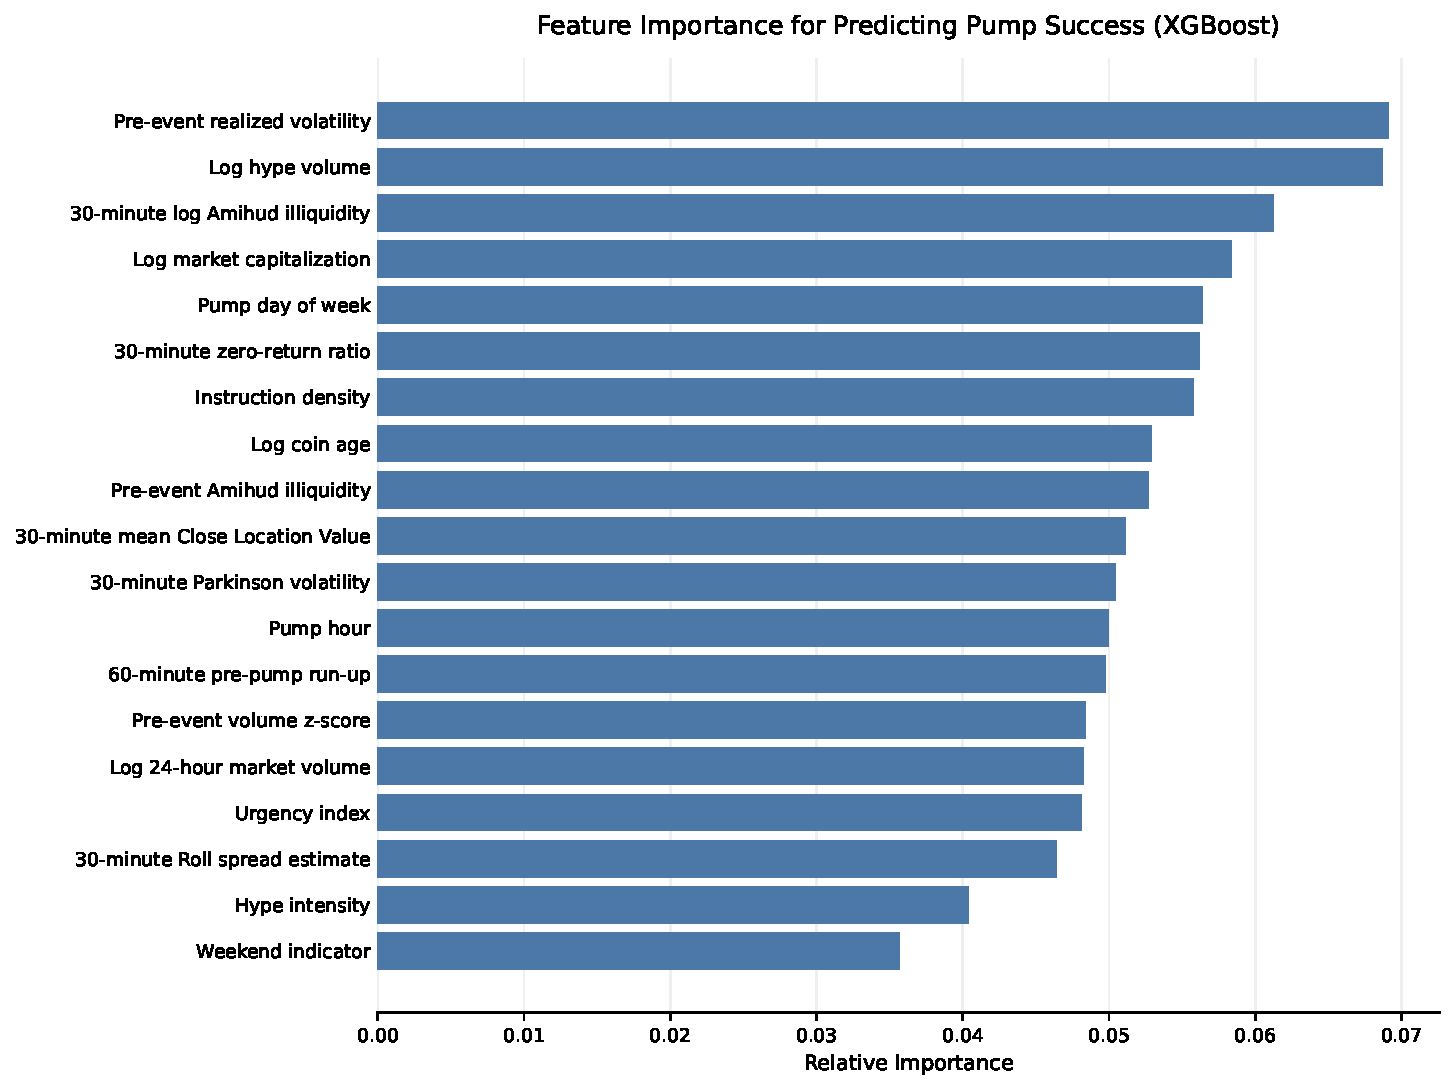
\includegraphics[width=0.78\textwidth,trim=0 0 0 7mm,clip]{figures/ch4/feature_importance_without_channel.pdf}
\datasetnote{Values are relative XGBoost feature-importance scores and should be read as predictive rankings, not causal estimates.}
\end{figure}

The two parts still support one broader interpretation. Pump outcomes are not random reactions to isolated messages. They are structured by the interaction between message design, asset characteristics, timing, and pre-reveal market conditions. The causal model focuses on a smaller set of theoretically motivated signal features, while the predictive model allows many variables to work together. This makes the predictive result useful as supporting evidence for structure in the data. It does not identify the mechanism by itself, but it shows that the conditions surrounding a pump contain information before the outcome is known.

The threshold analysis in Table~\ref{tab:threshold-optimization} gives the predictive result a practical meaning, but also shows why it should not be overstated. Raising the decision threshold increases precision and reduces the number of predicted positive events, while recall falls. This trade-off is useful for understanding model behavior, but it is not the same as a trading rule. In this thesis, \textit{Success} means only that the \textit{10-Minute Logarithmic Return} is positive. It does not mean that a trader could enter and exit at the right moments, avoid slippage, pay fees, and still realize a profit. The fixed 10-minute checkpoint is a standardized way to compare events, not a full measure of event profitability.

Several limits remain important for both the causal and predictive findings. The study is observational, and pump signals were not randomly assigned. Organizers may vary hype, urgency, or instruction density when they already expect a coin to move, or when they believe participants need stronger pressure. This means that signal style can reflect organizer expectations as well as influence participant behavior. The DML design reduces this problem by adjusting for observed pre-reveal conditions, but it cannot fully separate every strategic choice made before the signal. The E-value results in Table~\ref{tab:evalue-results} provide approximate sensitivity diagnostics for unmeasured confounding under the reported calculation, but they do not remove this concern. The small-cap urgency result has stronger sensitivity support than some other significant estimates, yet it still depends on the model specification and the observed controls.

The use of \textit{Market Capitalization} also limits the interpretation. Chapter~\ref{ch:literature-framework} treats market capitalization as a practical proxy for market depth and vulnerability, not as a direct measure of order-book liquidity. This matters because two coins with similar capitalization can still differ in trading depth, exchange structure, spread, and active market participation. The result therefore supports a market-cap boundary condition, but future work with richer order-book data could test the same mechanism more directly.

Finally, the grouped holdout design reduces direct dependence on \textit{Channel ID}, but it cannot fully remove organizer patterns. Figure~\ref{fig:channel-returns-distribution} shows that outcomes differ across Telegram groups, even though many large channels remain close to zero in median return. Channels may repeatedly choose similar coins, exchanges, timings, or message styles, and these habits can still appear indirectly through other variables. This limitation should be kept in mind when reading the predictive results, because the grouped holdout design tests generalization across observed channels rather than across all possible pump settings.
